\chapter{Results}
\label{ch:res}

In this chapter, we examine the strength of our proposed algorithms and compare TD-Stem($\lambda$) with TD-Leaf($\lambda$) in specific. We do this by considering end games with no more than 3 pieces on the board. By limiting ourselves to these kinds of problems we can perform objective comparisons with the metrics discussed in previous chapter. The first experiment in section \ref{sec:krk} deals with a \gls{krk} endgame. An additional experiment with different hyper-parameters is carried out in section \ref{sec:kqk}. Finally, a more generalized piece setup is used for the simulations discussed in \ref{sec:3p}.

\section{Experiment 1: king rook king with uniform sampling}
\label{sec:krk}

The first simulations we ran were all on the \gls{krk} endgame, where the obvious goal for the player holding the rook is to checkmate the opponent as efficiently as possible. To facilitate the process, we started by only giving the white side the rook. If the game ends in a draw, white receives a negative reward:
\begin{equation*}
\label{eq:rexp1}
r(s_t,a_t) = \begin{cases} 
   10 & \text{if } s_{t+1} \textnormal{ is checkmate}\\
   -10 & \text{if } s_{t+1} \textnormal{ is draw} \\
   0 &  \textnormal{else}
  \end{cases}
\end{equation*}
The initial starting positions in this simulation were set by randomly placing the kings and rook on the board under the constraint of being a legal position, ensuring to be totally unbiased. The value network did not contain any convolutional layers yet, only a fully connected layer with 128 hidden units as shown in figure \ref{fig:fnn}.\\


\begin{figure}
\centering
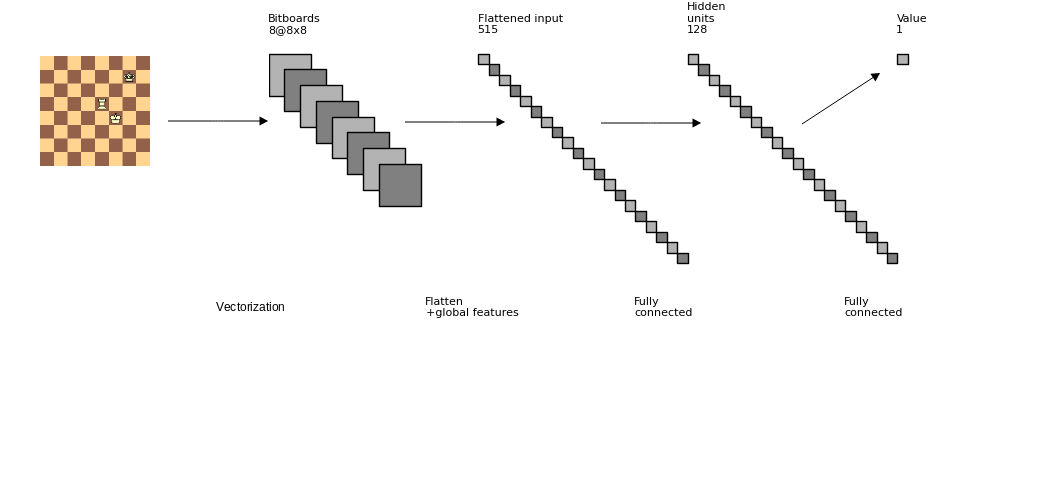
\includegraphics[trim={0 6cm 0 0cm},clip,scale=0.5]{fig/arch/fc}
\caption[\gls{nn} used in the first experiment]{Depiction of the \gls{nn} used in the first experiment. The binary input features are fed into a 1 layer \gls{fnn}.}
\label{fig:fnn}
\end{figure}

We ran the simulation script on machine A (section \ref{subsec:software}) over 7 stages identical for both TD-Leaf($\lambda$) and TD-Stem($\lambda$) with a learning rate $\alpha=10^{-4}$. The hyper parameters during the stages are laid out in table \ref{tab:exp1}. Furthermore, $M=50$ and $f_\epsilon(i)=(i)^{-3/4}$. Since samples are uniformly distributed, $R=0$. $K$ and $d_r$ were not implemented yet.\\

The resulting learning curve from figure \ref{fig:lc} gives the impression that our variant outperforms the state of the art TD-learning algorithm. One could argue that the 2nd and 3th stage have not induced additional learning. We also notice how increasing the depth boosts training. 

We prove this to be true by letting a greedy agent perform 2000 episodes with both methods against a perfect player using the \gls{krk} tablebase as reference. With the value function learned in TD-Stem($\lambda$), we succeed at winning about 85\% of the positions, clearly outperforming TD-Leaf($\lambda$). When winning, both techniques seem equally good. When the engine is at the losing side, it defends itself better with our variant. The reason why TD-Leaf($\lambda$) evaluates moves faster during self play, is because it has more difficulties finding wins (remember from section \ref{subsec:selfplay} how the iteration continues until enough rewards have been collected).\\

Let us observe the bar plots (figure \ref{fig:krk_perf}) in function of the theoretical \gls{dtm} to study which positions the generated models can solve. Aside of showing the superiority of TD-Stem($\lambda$) in this experiment, it indicates how TD-Learning propagates information further and further from the terminal states where the rewards are awarded. Training may have stopped somewhat early, as the winning rate of the model was still improving.\\

If we investigate the value function in figure \ref{fig:krk_vf}, we understand why the model does not always succeed at making progress and approaching checkmate. Notice how the variance increases the further we go from a winning terminal state, indicating that although the average value function contains the right trend, we have not found enough solutions yet for these though positions. \\
We also observe that especially close to checkmate, the variance in TD-stem($\lambda$) is way smaller than in TD-leaf($\lambda$).

\begin{table}[]
\centering
\caption{Hyper-parameters of the stages in Experiment 1}
\label{tab:exp1}
\begin{tabular}{r|rrrrr}
\textbf{Stage} & \textbf{$N$}  & \textbf{$I$} & \textbf{$d_V$} & \textbf{$\lambda$}& \textbf{$i_0$} \\ \hline
1     & 5000 & 20  & 1     & 0.5  & 1     \\
2     & 5000 & 20  & 1     & 0.5  & 2     \\
3     & 5000 & 20  & 1     & 0.7  & 2     \\
4     & 500  & 20  & 3     & 0.8  & 2     \\
5     & 250  & 30  & 3     & 0.8  & 2     \\
6     & 250  & 30  & 3     & 0.8  & 2     \\
7     & 250  & 50  & 3     & 0.8  & 2    
\end{tabular}
\end{table}

\begin{table}[]
\centering
\caption{Performance comparison TD-Leaf($\lambda$) and TD-Stem($\lambda$)}
\label{tab:perf_krk}
\begin{tabular}{l|rr}
    & \multicolumn{1}{l}{\textbf{TD-Leaf($\lambda$)}} & \multicolumn{1}{l}{\textbf{TD-Stem($\lambda$)}} \\ \hline
\textbf{WCR} & 0.48                                   & \textbf{0.85}                          \\
\textbf{WE}  & \textbf{0.87}                          & 0.86                                   \\
\textbf{LHS} & 0.80                                   & \textbf{0.91}                          \\
\textbf{MPS} & \textbf{228}                           & 205                                    \\
\textbf{N }  & 353 500                                & \textbf{304 500}                      
\end{tabular}
\end{table}

\begin{figure}
\centering
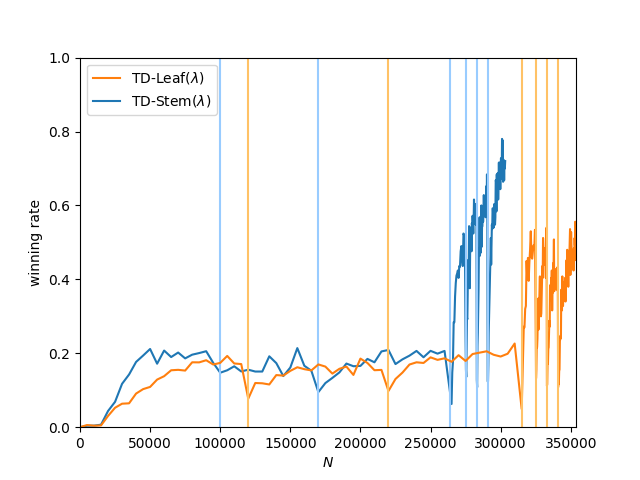
\includegraphics[scale=0.5]{fig/plots/krk_lc}
\caption[Learning curve experiment 1]{The learning curve of the experiment. The vertical lines indicate when the stages start.}
\label{fig:lc}
\end{figure}

\begin{figure}
\centering
\begin{subfigure}[b]{0.4\textwidth}
\centering
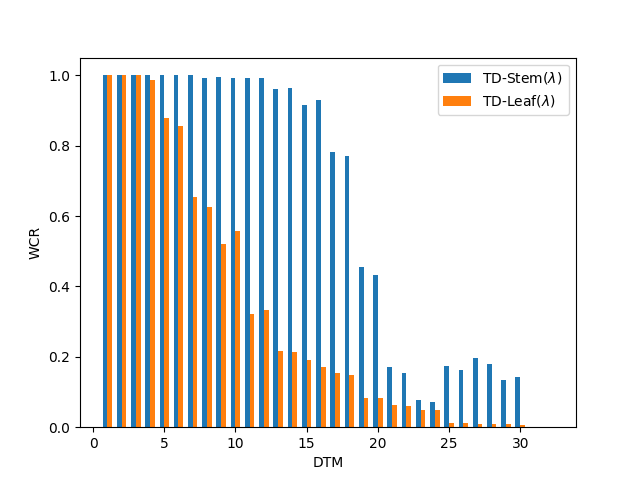
\includegraphics[scale=0.5]{fig/plots/krk_wcr}
\caption{win conversion rate \gls{krk} endgame}
\end{subfigure}
\\
\begin{subfigure}[b]{0.4\textwidth}
\centering
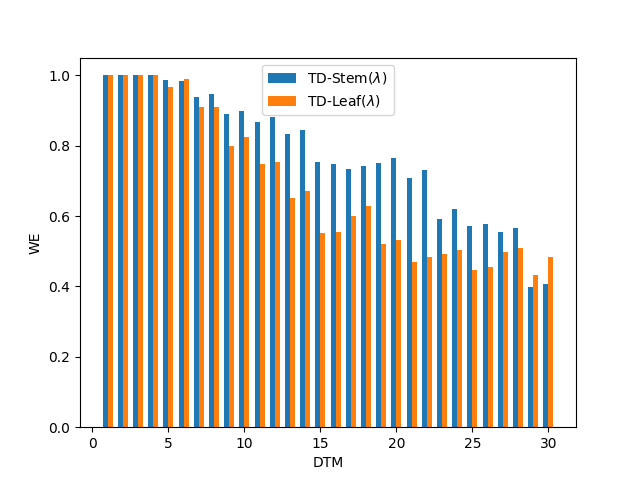
\includegraphics[scale=0.5]{fig/plots/krk_we}
\caption{win efficiency \gls{krk} endgame}
\end{subfigure}
\qquad
\begin{subfigure}[b]{0.4\textwidth}
\centering
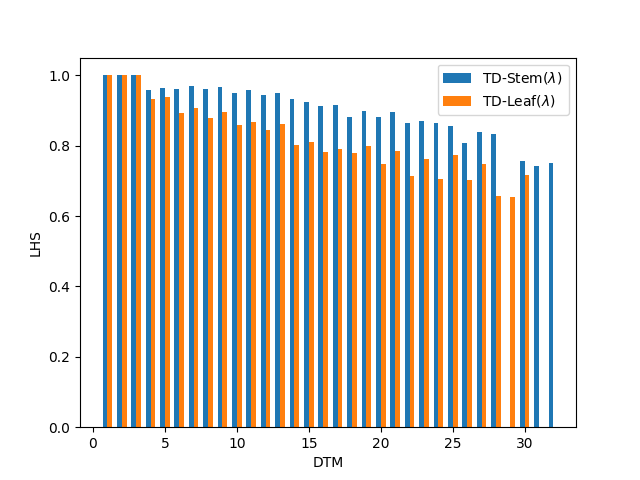
\includegraphics[scale=0.5]{fig/plots/krk_lhs}
\caption{loss holding score \gls{krk} endgame}
\end{subfigure}
\caption[Performance comparison between TD-Stem($\lambda$) and TD-Leaf($\lambda$) experiment 1]{Performance comparison between TD-Stem($\lambda$) and TD-Leaf($\lambda$) through the form of bar charts with respect to the theoretical \gls{dtm}. These bar plots are obtained by playing a trained model 2000 positions from a validation set against an optimal player and storing all encountered positions together with the final outcome.}
\label{fig:krk_perf}
\end{figure}

\begin{figure}
\centering
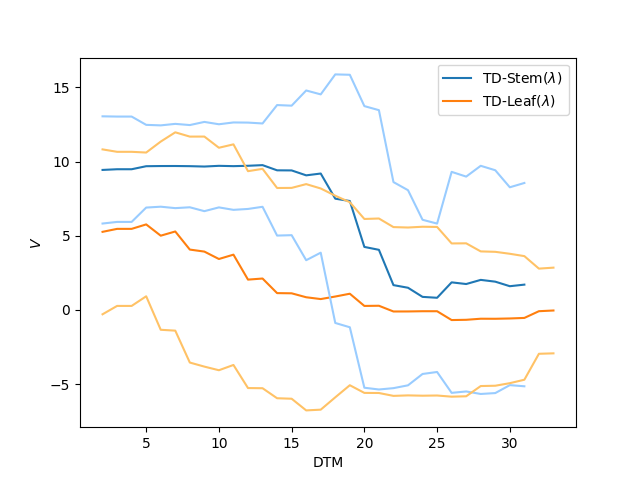
\includegraphics[]{fig/plots/krk_vf}
\caption[value curve experiment 1]{Value curve showing the average value estimate of over 15000 \gls{krk} positions. To visualize the variance over these values, the 95\% intervals are provided as well.}
\label{fig:krk_vf}
\end{figure}

\section{Experiment 2: king queen king with sampling from dataset}
\label{sec:kqk}
In this section, we try to confirm our conjecture of TD-Leaf($\lambda$) being at least equivalent to TD-Stem($\lambda$) in performance by analyzing an even easier problem, the \gls{kqk} endgame. In contrast to experiment 1, both white and black can possess the queen. This trait makes the value function harder to learn, but is necessary as the goal should be to learn a symmetrical value function (remember the zero-sum property). To enforce this characteristic, data augmentation is performed as described in section \ref{subsec:selfplay}.\\
Another main difference with experiment 1 is the sampling of initial positions, which happens by randomly picking boards from a dataset. In addition 5 random moves are made on these initial states with the goal of reaching an as diverse set of games as possible, which should encourage generalization by the learning algorithm.\\

To experiment with the idea of learning good bitboard representations, the value network is a \gls{cnn} as designed in figure \ref{fig:cnn1}. The use of $(1,1)$ patches for the convolutional layer can be interpreted as an attempt to learn the most important squares with respect to the problem, given the piece locations and mobilities. The applied learning rate is $\alpha=10^{-6}$. As in experiment 1, the maximal number of moves per episode is $M=50$. However, we have changed the policy to a linear decay approach: $f_{\epsilon}(i)=1-0.02i$. Changes in between the stages are represented in table \ref{tab:exp2}. For this experiment, all simulations were ran on machine B (section \ref{subsec:software}).\\

\begin{table}[]
\centering
\caption{Hyper-parameters of the stages in Experiment 2}
\label{tab:exp2}
\begin{tabular}{r|rrrrrr}
\textbf{Stage} & \textbf{$N$}  & \textbf{$I$} & \textbf{$d_V$} & \textbf{$\lambda$}& \textbf{$i_0$} & $K$ \\ \hline
1     & 500 & 20  & 1     & 0.5  & 0 & 10    \\
2     & 250 & 20  & 3     & 0.6  & 20 & 20    \\
3     & 250 & 20  & 3     & 0.7  & 40 & 30    \\
4     & 250  & 50  & 3     & 0.8  & 40 & 30    \\
5     & 250  & 20  & 3     & 0.8  & 45 & 30       
\end{tabular}
\end{table}

\begin{figure}
\centering
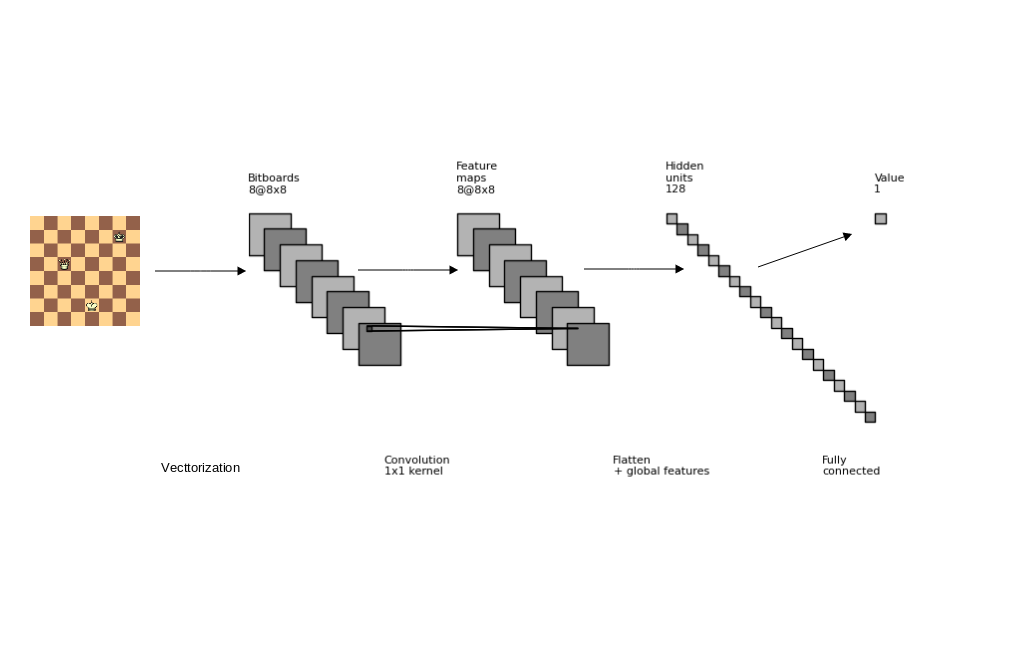
\includegraphics[trim={0 6cm 0 6cm},clip,scale=0.5]{fig/arch/cnn1}
\caption[\gls{cnn} architecture deployed in experiment 2]{The (relatively simple) \gls{cnn} architecture deployed in experiment 2.}
\label{fig:cnn1}
\end{figure}

A first glance at the learning curve in figure \ref{fig:lc_kqk} can trick one in believing that TD-Leaf($\lambda$) learns quicker than TD-Stem($\lambda$). However, the sudden dive from the curve starting from episode 30000 corresponding with TD-Leaf($\lambda$) hints to a contrary belief. An explanation for this behavior is that the winning rate in the plot represents the agent's strength against itself, and not against the optimal agent. Hence, the decrease is a sign of an improvement at the losing side. In retrospect, we are able to notice the exact same effect in experiment 1 in figure \ref{fig:lc} around episode 330000. This idea is backed up by the fact that the strength of the models \footnote{The metrics in experiment 2 have been measured in a similar fashion as experiment 1.} was already analyzed after termination of the third stage. Performances of both models against the optimal player were so much worse than what the learning curve indicated, that two stages were added to the process. These result in a big improvement in play as shown in table \ref{tab:perf_kqk}. As TD-Stem($\lambda$) does not appear to contain this subtle effect, we believe it to be probably faster in general, and more certainly it succeeds at improving the winning and losing side at the same time while TD-Leaf($\lambda$) appears to improve the players one after another.\\
In table \ref{tab:perf_kqk} and figure \ref{fig:kqk_perf} it can be noticed how more equilibrated the performances of both models are in comparison to previous experiment. However, TD-Stem($\lambda$) continues to outperform the state of the art with respect to the \gls{lhs}, advocating in favor of our argument that TD-Stem($\lambda$) improves both sides at the same time.\\
A possible explanation for this effect could be the following. If we review the mechanism behind TD-Leaf($\lambda$) (section \ref{subsec:tdleaf}), we can notice how the final outcome of the game influences the update. However, we may be updating  leaf nodes we have never encountered in the simulation. This is in contrast with TD-Stem($\lambda$), where the game states are used as training samples.
The insight that the states used for the network update provide a true evidence about their value (namely, the outcome of the played game) can be an explanation for this effect. On the contrary, TD-Leaf($\lambda$) updates states seen in search, not necessarily in simulation, can result in updates in the direction of a 'wrong belief', as the final outcome participates to the equation (see section \ref{subsec:tdleaf}).\\

The value curves (figure \ref{fig:kqk_vf}) indicate how the variance is higher for increasing \glspl{dtm}.

\begin{figure}
\centering
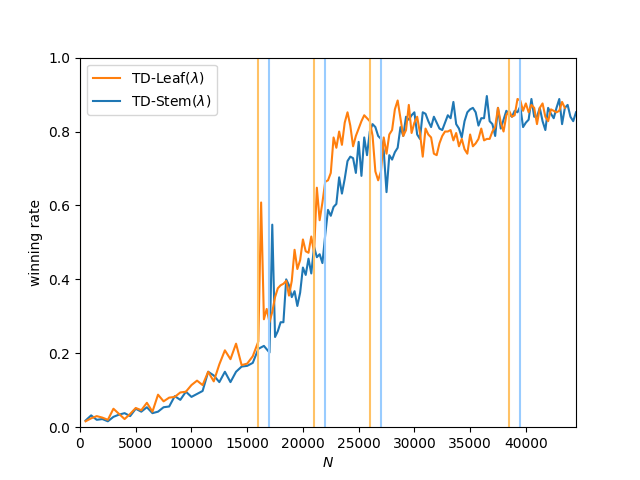
\includegraphics[scale=0.8]{fig/plots/kqk_lc}
\caption[Learning curve of the second experiment]{The learning curve of the second experiment, divided in 5 stages.}
\label{fig:lc_kqk}
\end{figure}


\begin{table}[]
\centering
\caption{Performance comparison TD-Leaf($\lambda$) and TD-Stem($\lambda$)}
\label{tab:perf_kqk}
\begin{tabular}{l|rr|rr}
& \multicolumn{2}{c|}{\textbf{3 stages}} & \multicolumn{2}{c}{\textbf{5 stages}} \\

    &\multicolumn{1}{l}{\textbf{TD-Leaf($\lambda$)}} & \multicolumn{1}{l|}{\textbf{TD-Stem($\lambda$)}}&\multicolumn{1}{l}{\textbf{TD-Leaf($\lambda$)}} & \multicolumn{1}{l}{\textbf{TD-Stem($\lambda$)}} \\ \hline
\textbf{WCR} & 0.65 & \textbf{0.77} & 0.90                                  & 0.90                          \\
\textbf{WE} & \textbf{0.67} & 0.64 & 0.89                          & 0.89                                   \\
\textbf{LHS} & 0.89 & 0.89 & 0.95                                   & \textbf{0.97}                          \\
\textbf{MPS} & 346 & \textbf{359} & 180                           & \textbf{188}                                    \\
\textbf{N } & \textbf{26000} & 27000  & \textbf{43500}                                & 44500                      
\end{tabular}
\end{table}


\begin{figure}
\centering
\begin{subfigure}[]{0.4\textwidth}
\centering
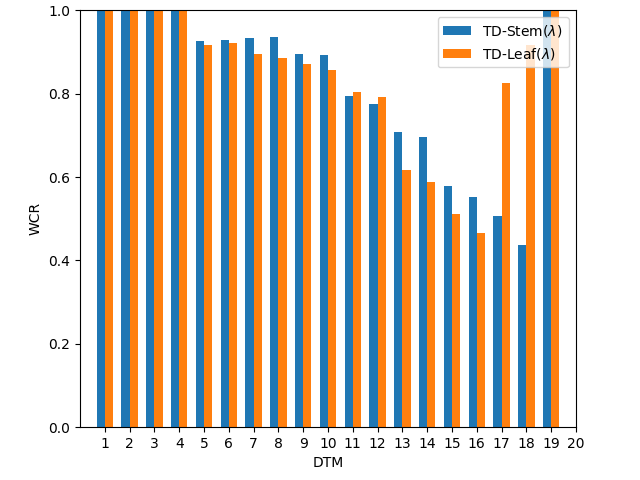
\includegraphics[scale=0.45]{fig/plots/kqk_wcr}
\caption{win conversion rate \gls{kqk} endgame}
\end{subfigure}
\\
\begin{subfigure}[]{0.4\textwidth}
\centering
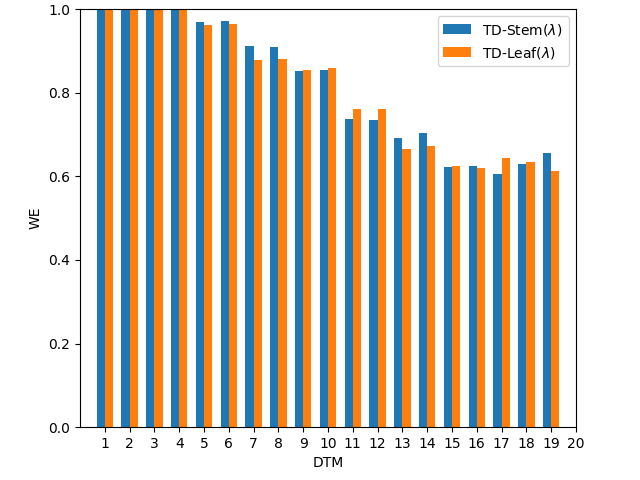
\includegraphics[scale=0.45]{fig/plots/kqk_we}
\caption{win efficiency \gls{krk} endgame}
\end{subfigure}
\qquad
\begin{subfigure}[]{0.4\textwidth}
\centering
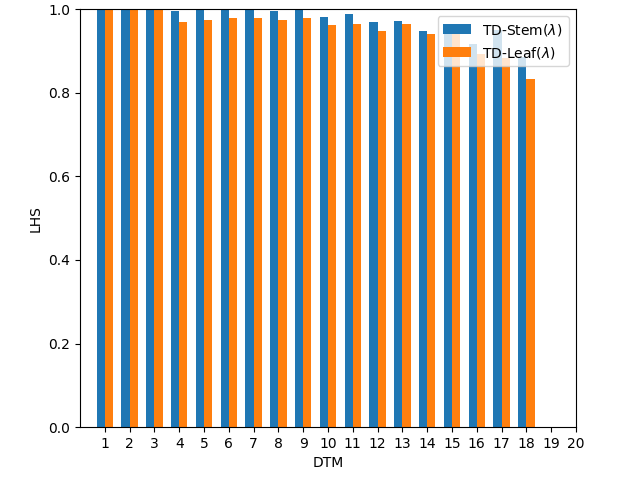
\includegraphics[scale=0.45]{fig/plots/kqk_lhs}
\caption{loss holding score \gls{krk} endgame}
\end{subfigure}
\caption[Performance comparison between TD-Stem($\lambda$) and TD-Leaf($\lambda$)]{Performance comparison between TD-Stem($\lambda$) and TD-Leaf($\lambda$) through the form of bar charts with respect to the theoretical \gls{dtm}.}
\label{fig:kqk_perf}
\end{figure}

\begin{figure}
\centering
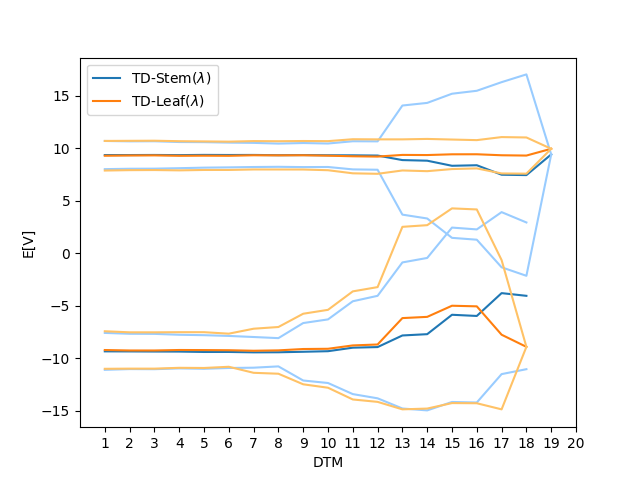
\includegraphics[]{fig/plots/kqk_vf}
\caption[Value curves experiment 2]{Value curves for positions where white ($E[V]>0$) and black ($E[V]<0$) hold the queen.}
\label{fig:kqk_vf}
\end{figure}

\section{Experiment 3: 3 pieces endgames with sampling from dataset} 
\label{sec:3p}

In this experiment, we look at a much more complex problem, namely end games where every configuration is trained with 3 pieces on the board. Hence, the possible chess positions are:
\begin{itemize}
\item \gls{kqk}
\item \gls{krk}
\item \gls{kbk}
\item \gls{knk}
\item \gls{kpk}
\end{itemize}
From which \gls{knk} and \gls{kbk} are less relevant as they are categorized in terminal states (these positions are a draw due to insufficient material). As all piece types are seen in the dataset, the amount of bitboards in the input is now 24. As the problem seems much more complex, a deeper network was deployed as laid out in figure \ref{fig:deep}. One of the reasons this problem is much harder is that \gls{kpk} endings can only be won after promotion. Additionally, many cases exist where it is impossible to force a pawn promotion when the opponent plays perfectly. The training setup was equivalent to the previous experiments, now with the hyper-parameters set as shown in table \ref{tab:exp3}.\\
\begin{figure}
\centering
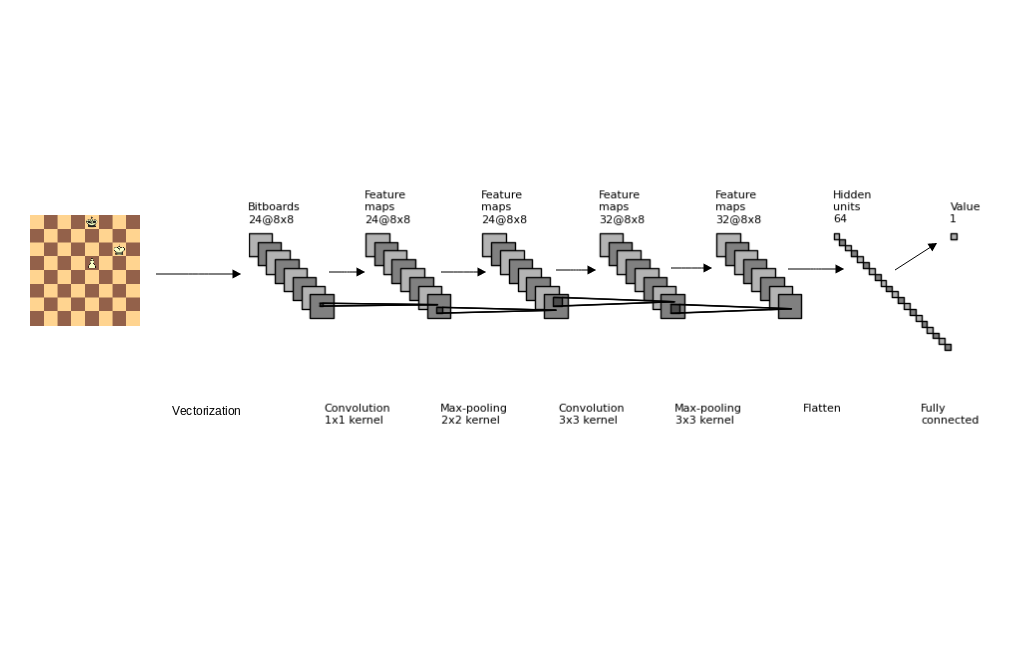
\includegraphics[trim={0 6cm 0 6cm},clip,scale=0.45]{fig/arch/deep}
\caption[\gls{cnn} architecture deployed in experiment 2]{The (relatively simple) \gls{cnn} architecture deployed in experiment 2.}
\label{fig:deep}
\end{figure}

\begin{table}[]
\centering
\caption{Hyper-parameters of the stages in Experiment 2}
\label{tab:exp3}
\begin{tabular}{r|rrrrrrr}
\textbf{Stage} & \textbf{$N$}  & \textbf{$I$} & \textbf{$d_V$} & \textbf{$\lambda$}& \textbf{$i_0$} & $K$ & $d_R$ \\ \hline
1     & 250 & 100  & 1     & 0.5  & 0 & 100 & 3   \\
2     & 250 & 100  & 3     & 0.7  & 50 & 100  & 5  \\
3     & 250 & 60  & 3     & 0.7  & 95 & 100  & 5  \\
4     & 250  & 100  & 3     & 0.8  & 95 & 100 & 5   \\
5     & 250  & 100  & 3     & 0.8  & 95 & 100 & 5    \\ 
6     & 250  & 80  & 3     & 0.7  & 95 & 100 & 5    \\ 
7     & 250  & 100  & 3     & 0.7  & 95 & 100 & 5    \\  
\end{tabular}
\end{table}

As one can see in table \ref{tab:perf_3p}, the progress from stage 4 onwards is not satisfactory. Multiple reasons serve to explain this:
\begin{itemize}
\item One reason could be that more episodes should have been simulated before increasing the depth to $d_V=3$. Additionally, the fact that many data have been thrown away due to the slow simulations when too much samples were used as training set could have had an influence. One of the powers of TD learning is the correlation between successive samples, and we might have decorrelated too much for this problem. It is also known that deep networks only have the tendency to generalize well when enough data have been seen.
\item Another reason could be that the error surface is less smooth due to the more varied piece setups, which results in getting stuck in local minimums.
\item Finally, it could be that the trained model tends to improve when playing more episodes. Possibly by generating games with a higher search depth. The problem is that simulating episodes is already slow when $d_V=3$.
\end{itemize}

It should be studied further how these board setups could be learned through self play only without additional bias. Our opinion is that throwing less data away, albeit having much slower experiments, is the way to go. Unfortunately, there was insufficient time left at this point in the master thesis to do further research in this direction.

\begin{table}[]
\centering
\caption{Performance of the trained model in experiment.}
\label{tab:perf_3p}
\begin{tabular}{l|rr|rr}
& \multicolumn{2}{c|}{\textbf{3 stages}} & \multicolumn{2}{c}{\textbf{7 stages}} \\

    &\multicolumn{1}{l}{\textbf{TD-Leaf($\lambda$)}} & \multicolumn{1}{l|}{\textbf{TD-Stem($\lambda$)}}&\multicolumn{1}{l}{\textbf{TD-Leaf($\lambda$)}} & \multicolumn{1}{l}{\textbf{TD-Stem($\lambda$)}} \\ \hline
\textbf{WCR} &\textbf{0.32} & 0.30 & 0.30                                  & 0.30                          \\
\textbf{WE} & \textbf{0.86} & 0.92 & 0.83                          & 0.85                                   \\
\textbf{LHS} & 0.78 &\textbf{ 0.80} & 0.78                                   & \textbf{0.79}                          \\
\textbf{MPS} & \textbf{39} & 38 & 19                           & 19                                    \\
\textbf{N } & \textbf{133500} & 135000  & \textbf{183500}                                & 186000                     
\end{tabular}
\end{table}

\section{Conclusion}

By doing these experiments we have learned several things. First of all, it seems that we have found a worthy and at least equivalent method for the state of the art TD learning algorithm in TD-Stem($\lambda$). We discussed two possible explanations why our variant may be an improvement over TD-Leaf($\lambda$): depth is included in the estimated value function and all effective outcomes correspond to an encountered board position. Secondly, in the experiments where we fixed the piece configuration to \gls{krk} and \gls{kqk}, the final models were able to solve the problems up until a decent level purely through self play and supervised learning. Lastly, we found that more complex variations where more configurations should be learned all at once are a bigger deal. This may be solved by using more training data and increasing the depth of search during self play at the cost of simulation speed. This is still open for examination in future research.
